%
% LaTeX
%
\pagebreak
\section{Beweise zum Strukturpolynom}\label{se:Anhang}


\begin{theorem}[Strukturpolynom von Multiplikation und Addition]
Seien $E_0$ und $E_1$ Ausdrücke,
sei $\circ$ eine Operation $\in\{+,\times\}$
und seien
\begin{equation*}
  p_{E_0}(z) = \prod_{k=1}^{N_0} (z-z_{0,k}) = \sum_{k=0}^{N_0} c_{0,k} z^k
  ,\quad
  z\in\C,z_{0,k}\in\A,\;c_{0,k}\in\Q
\end{equation*}
bzw. 
\begin{equation*}
  p_{E_1}(z) = \prod_{k=1}^{N_1} (z-z_{1,k}) = \sum_{k=0}^{N_1} c_{1,k} z^k
  ,\quad
  z\in\C,z_{1,k}\in\A,\;c_{1,k}\in\Q
\end{equation*}
die zugehörigen Strukturpolynome 
mit algebraischen Nullstellen $z_{0,k}$ bzw. $z_{1,k}$
und rationalen Koeffizienten $c_{0,k}$ bzw. $c_{1,k}$.
Dann hat das Strukturpolynom
\begin{equation*}
  p_{E_0\circ E_1}(z) = \prod_{k_0=1}^{N_0}
                        \prod_{k_1=1}^{N_1}
                        (z-(z_{0,k_0}\circ z_{1,k_1}))
                      = \sum_{k=0}^{N_0N_1} c_{\circ,k} z^k
\end{equation*}
des Ausdrucks $E_0\circ E_1$ ebenfalls rationale Koeffizienten $c_{\circ,k}\in\Q$.
\begin{proof}
\cite{BFMS} enthält einen Beweis für den Fall ganzzahliger Koeffizienten,
der auf rationale Koeffizienten übertragen werden kann.
\end{proof}
\end{theorem}


\begin{theorem}[Strukturpolynom des Kehrwerts]
Sei $E$ ein Ausdruck und sei
\begin{equation*}
  p_E(z) = \prod_{k=1}^N (z-z_k) = \sum_{k=0}^N c_k z^k
  ,\quad
  z\in\C,z_k\in\A,\;c_k\in\Q
\end{equation*}
das Strukturpolynom des Ausdrucks $E$ mit rationalen Koeffizienten $c_k$.
Dann hat das Strukturpolynom
\begin{equation*}
  p_{1\div E}(z) = \prod_{k=1}^N \left(z-(1\div z_k)\right)
                 = \sum_{k=0}^N c_{\div,k} z^k
  ,\quad
  c_{\div,k}\in\Q
\end{equation*}
des Ausdrucks $1\div E$ ebenfalls rationale Koeffizienten $c_{\div,k}$.
\begin{proof}
Das Polynom
\begin{equation*}
  z^N
  p_E(z^{-1}) = z^N\sum_{k=0}^N c_k z^{-k}
              =    \sum_{k=0}^N c_k z^{N-k}
              =    \sum_{k=0}^N c_{N-k} z^k
\end{equation*}
hat dieselben Koeffizienten wie $p_E(z)$,
nur in umgekehrter Reihenfolge.
Daher sind die Koeffizienten des Polynoms 
$z^N p_E(z^{-1})$ rational.
Nun gilt für dasselbe Polynom auch
\begin{equation*}
  z^N p_E(z^{-1}) 
  = 
  z^N \prod_{k=1}^N (z^{-1}-z_k)
  =
  c_0\,(-1)^N \prod_{k=1}^N (z-z_k^{-1}),
\end{equation*}
weshalb die Koeffizienten $c_{\div,k}$ des Polynoms
\begin{equation*}
  p_{1\div E}(z) = \prod_{k=1}^N (z-(1\div z_k))
                 = \sum_{k=0}^N c_{\div,k} z^k
\end{equation*}
ebenfalls rational sind. 
\end{proof}
\end{theorem}


\pagebreak
\section{$N^{\rm th}$ band filter}\label{se:AnhangFilter}

Prototypfilter für die Übertragungsfunktionen 
der Analyse-Resynthese-Kanäle einer 
perfekt rekonstruierenden Polyphasenfilterbank. 

\begin{figure}[H]
\centering
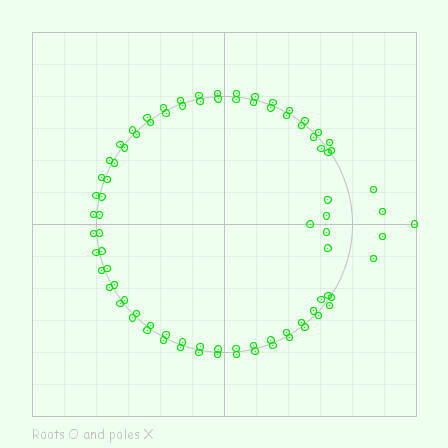
\includegraphics[width=83mm]{images/Figure_roots4.png}
\caption{Nullstellen}
\end{figure}

Die Nullstellen treten paarweise auf, 
und das Produkt eines jeden Paares
hat den Betrag $1$.

\begin{figure}[H]
\centering
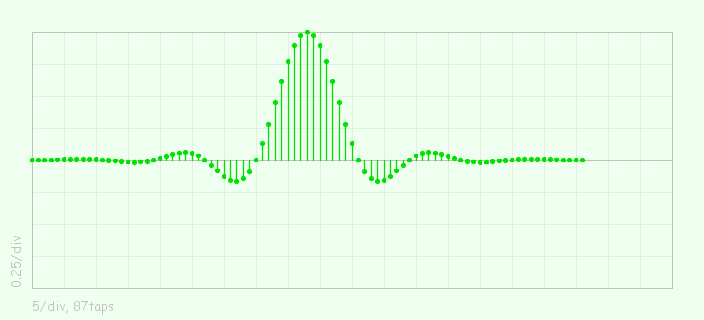
\includegraphics[height=23mm]{images/Figure_cfnbir.png}
\hspace{10mm}
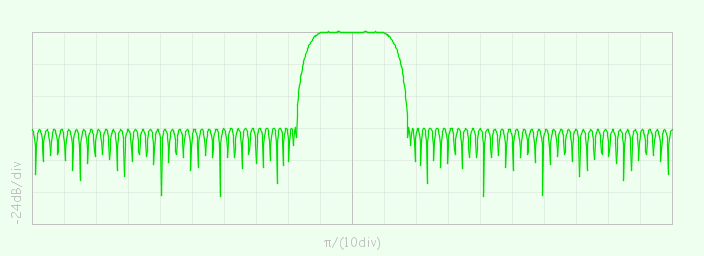
\includegraphics[height=23mm]{images/Figure_cfnbPolished.png}
\caption{Impulsantwort, Frequenzgang}
\end{figure}

%
% EOF
%
